\documentclass[10pt]{article}

\usepackage[T1]{fontenc}
\usepackage{lmodern}
\usepackage[margin=1in]{geometry}
\usepackage{microtype}
\usepackage{amsmath,amssymb}
\usepackage{booktabs}
\usepackage{graphicx}
\usepackage{xcolor}
\usepackage[numbers,sort&compress]{natbib}
\usepackage[hidelinks]{hyperref}
\usepackage{url}

\setlength{\parskip}{0.4em}
\setlength{\parindent}{0pt}
\renewcommand{\arraystretch}{1.1}
\setlength{\emergencystretch}{2em}

\newcommand{\ie}{i.e.\ }
\newcommand{\eg}{e.g.\ }
\newcommand{\bs}{\textbackslash}

\title{Trutina: Typed Decision Probabilities from a 4B Language Model\\with Letter Readout and Trainable Early Exits}
\author{Xinyuan Weng\\[2pt]\small Aldine Labs\\\small \texttt{inbound@aldine.cn}}
\date{}

\begin{document}
\maketitle

\begin{abstract}
Typed decision models answer a question about a state with a probability for every option instead of generating text.
We present Trutina 4B, a decision model built on Qwen3.5-4B that reads the answer from the LM-head logits of the option letters at a fixed position, after a rank-16 LoRA fine-tune of all linear layers.
Four design choices carry most of the result.
First, presenting the question before and after the input raises zero-shot accuracy by 3 to 4 points on a backbone that is mostly linear attention.
Second, a two-round tournament extends the letter readout to 255 options without new parameters.
Third, affine exits at layers 12, 16, 20 and 24, distilled from the final layer with detached inputs, let a request stop at a confidence threshold and otherwise continue from where it stopped.
Fourth, continued training with a high share of replay adds new capabilities without forgetting.
We also report that a decision head newly trained on hidden states scored 74.0\% on the JevBench public set, below the 79.7\% of the untrained backbone's letter readout, which led us to abandon it.
At full depth the model reaches 87.4\% on the 231 JevBench public tasks and 74.65\% accuracy (KL 0.156) on the zero-shot LocalLLaMA typed-decisions test set.
The adaptive mode uses 21.6 of 32 layers on average at 86.6\%, with a median latency of 14.0~ms on one RTX PRO 6000.
Among six open 4B decision models run under one protocol, it has the highest accuracy on three of eight evaluations and is weaker on hard multi-step judgements.
Weights and code are released under Apache-2.0.
\end{abstract}

\section{Introduction}

A decision model receives a state, such as a document, a log or a screenshot, together with typed questions, and returns a probability for each option.
Three question types are supported: yes/no, choice among 2 to 255 options, and score over 2 to 10 ordered levels.
Compared with a chat model that writes its answer as text, a decision model needs a single forward pass, its outputs can be thresholded directly, and it costs less in latency and compute.
The goal of this work is the best result within the 4B parameter class; outperforming larger models was not a goal.

We built Trutina 4B in five days, from the first survey to the release of the final version, using one laptop (Apple M5 Pro) for the first experiments and rented B200 GPUs for the training runs.
The first design, a new decision head trained on frozen-backbone hidden states, did not work (Section~\ref{sec:neg}).
The final design is simpler: the language-model head of a post-trained backbone is read at the position of the option letters, and everything else is training and inference machinery around that readout.

\paragraph{Contributions.}
\begin{itemize}
\item An audit showing that, when all options are visible, the pretrained LM head is a stronger prior than a newly trained decision head, with the corresponding zero-shot and training ablations (Sections~\ref{sec:readout} and~\ref{sec:ablate}).
\item A tournament readout that handles up to 255 options with letters A to Z only, and is 19.9 points more accurate than two-letter labels in a zero-shot test (Section~\ref{sec:tournament}).
\item Trainable intermediate exits in the form of a tuned lens, distilled with detached inputs and calibrated per exit, which allow adaptive depth with one stopping threshold (Section~\ref{sec:exits}).
\item A controlled comparison of training data for hard algorithmic questions, and an analysis of forgetting in continued training (Section~\ref{sec:training}).
\item A calibration analysis contrasting soft-label and hard-label probabilities, and an optional monotone map for yes/no questions (Section~\ref{sec:calib}).
\item An evaluation under one protocol against open 4B decision models, a paired comparison of successive versions, a contamination scan, and a record of negative results (Sections~\ref{sec:eval} and~\ref{sec:neg}).
\end{itemize}

\section{Related work}

\paragraph{Decision models.}
Decision models return typed probabilities instead of text. The System One interface of Jev~\cite{jev} popularised the task, and open systems built on small backbones followed, among them Plumb-4B~\cite{plumb}, JevK5~\cite{jevk5}, decider-4b~\cite{decider4b}, Sieve-4B~\cite{sieve}, spark-s1~\cite{spark}, SemIf~\cite{semif} and Liquid AI's d1~\cite{d1}. The study of LLM-as-Jev~\cite{llmjev} analyses number readouts, an anchor KL and the effect of short training data. Our work differs in reading the original LM head and in the exit mechanism.

\paragraph{Prompt order and repetition.}
For recurrent and linear-attention models, reading the question before the input and repeating it afterwards improves recall~\cite{arora,leviathan}. Our sandwich prompt applies the same idea to typed options.

\paragraph{Intermediate readouts and early exit.}
The logit lens~\cite{logitlens} and the tuned lens~\cite{tunedlens} read predictions from intermediate layers. Early-exit methods stop computation when a confidence criterion is met~\cite{calm,layerskip}. Our exits are affine tuned-lens maps distilled towards the final layer, and requests that do not stop continue from the saved hidden states.

\paragraph{Position bias.}
Multiple-choice answers depend on option order~\cite{pride,pine}, and permutation-averaged targets can distil this away~\cite{liusie}. We observe that the bias largely disappears after training and that permutation averaging adds nothing measurable (Section~\ref{sec:neg}).

\paragraph{Latent reasoning.}
Continuous latent reasoning, recurrent depth and pause tokens add computation without generating text~\cite{coconut,recdepth,pause}. Our attempt at a latent mode did not meet its criterion (Section~\ref{sec:neg}).

\paragraph{Calibration.}
Modern networks are over-confident, and temperature scaling is a standard remedy~\cite{guo}. We contrast temperatures fitted to soft labels with those fitted to hard labels.

\section{Task and evaluation protocol}
\label{sec:task}

A request contains a state and questions of three types: yes/no (the probability of yes), choice (2 to 255 options, one probability each) and score (a distribution over 2 to 10 ordered levels and its expected level).
Development relied mainly on JevBench v1.5~\cite{jevbench} and LocalLLaMA typed-decisions~\cite{localllama}, which score models in different ways.

JevBench is a community leaderboard whose downloadable public set has 231 tasks in easy (48), standard (72) and hard (111, of which 17 form the judge tier) tiers.
Its Intelligence score weights the public and sealed sets equally; the judge and hard tiers together carry 70\% of the weight; a yes/no answer with $P(\text{yes})$ between 0.2 and 0.8 counts as an abstention and is scored as wrong; score questions are graded by the normalised mean absolute error of the distribution's expected position; and choice questions use chance-corrected accuracy with expected calibration error (ECE)~\cite{guo} and the total variation distance to the gold distribution as calibration terms.
All JevBench figures in this paper are our own scoring of the public tasks, not official full-open-set or sealed-set results.

LocalLLaMA typed-decisions contains 400 cases and 2,000 questions (800 score, 600 choice, 600 yes/no) from four business workflows: agent-trace monitoring, customer support, invoices and security incidents.
Its gold labels are the mean of three samples at temperature 0.7 from a teacher model of about 4B parameters, so they are soft.
The dataset card gives reference points of 0.470 accuracy for answering by label frequency, 0.704 for perfect recovery of the generating latent factors and 0.735 for the teacher's agreement with itself.
Our training data contains none of these workflows, which makes the evaluation zero-shot.

DecisionBench~\cite{decisionbench}, this-that~\cite{thisthat}, JudgeBench~\cite{judgebench}, fast-decisions~\cite{fastdecisions}, MASSIVE~\cite{massive} and Decision Index 0.3~\cite{decisionindex} were used for evaluation only and never for training or weight selection.

\section{Method}

\subsection{Letter readout and the sandwich prompt}
\label{sec:readout}

The model is the post-trained Qwen3.5-4B~\cite{qwen35}.
Options are labelled (A) to (Z), and the prompt ends with \texttt{Best answer: (}; the probabilities are the softmax over the logits of the option letters at that position.
Yes/no questions are rendered as two options, and score levels are labelled in order.
The chat template is used with thinking disabled.
In the \emph{sandwich} format the questions and options appear once before and once after the state; when several questions share a state, the leading block contains all questions and the trailing copy only the current one, so that the state is encoded once per request.

We chose this format from zero-shot experiments covering two backbones (Base and post-trained), three orderings (state first, question first, sandwich) and two label styles (letters and numbers), scored on the JevBench public set, LocalLLaMA and a sample of 577 questions from our first validation split (Table~\ref{tab:readout}).

\begin{table}[t]
\centering\small
\caption{Zero-shot readout accuracy (\%) by backbone and ordering; letter labels. ``Post'' is the post-trained backbone with the chat template; Base uses plain text. Number labels differ by less than one point in no consistent direction.}
\label{tab:readout}
\begin{tabular}{lcccccc}
\toprule
 & \multicolumn{3}{c}{JevBench public} & \multicolumn{3}{c}{LocalLLaMA} \\
\cmidrule(lr){2-4}\cmidrule(lr){5-7}
Backbone & state first & question first & sandwich & state first & question first & sandwich \\
\midrule
Base & 73.2 & 68.4 & 77.1 & 47.8 & 52.4 & 59.9 \\
Post & 76.2 & 76.6 & \textbf{79.7} & 54.7 & 61.5 & \textbf{64.1} \\
\bottomrule
\end{tabular}
\end{table}

The sandwich raised JevBench by 3 to 4 points on both backbones and validation accuracy of the Base model by 7 points, the largest gain from any single change.
Of Qwen3.5's 32 layers, 24 use linear attention (Gated DeltaNet~\cite{gdn}).
A linear-attention layer that reads the state without knowing the question must compress it into a fixed-size memory that retains a little of everything; with the question first, the model knows what to retain, and the repetition at the end places the options next to the answer position.
This agrees with the findings on reading twice and on prompt repetition~\cite{arora,leviathan}.
The post-trained backbone is more accurate than Base (with the sandwich, $+2.6$ on JevBench and $+4.2$ on LocalLLaMA) but also more confident, and its KL on the soft-label sets is clearly worse (0.73 against 0.47 on LocalLLaMA), which training has to correct.

\subsection{Tournament readout for more than 26 options}
\label{sec:tournament}

The interface allows up to 255 options, while the model has seen only the letters A to Z in training.
Comparable systems use two-letter labels after Z or a 255-way linear head.
Our tournament divides the options, in their original order, into balanced groups of at most 26 and scores each group in its own forward pass.
The top $\lfloor 26/g\rfloor$ options of each of the $g$ groups go to a final round, which is scored once more.
A finalist's probability is $M$ times its final-round probability, where $M$ is the finalists' mean probability mass within their groups; the remaining options share $1-M$ in proportion to their group probabilities.
The model sees every option, only in different passes, and no parameter is added.

On MASSIVE~\cite{massive} (59 intents, 2,974 questions; not in the training data), a zero-shot comparison gives 59.4\% top-1 accuracy for two-letter labels (top-5 88.3\%) and 79.3\% for the two-round tournament (top-5 95.2\%); the reference of the answer plus 25 random distractors is 86.4\%.
When the answer comes after the label AA, two-letter labels reach 41.2\% and the tournament 80.0\%.
The time per question is 0.21~s against about 0.3~s on an L4 GPU.

\subsection{Trainable exits and adaptive depth}
\label{sec:exits}

Reading the LM head directly at an intermediate layer does not answer well.
Passing the residual stream of the untrained backbone at each layer through the final norm and the LM head (a logit lens~\cite{logitlens}) gives chance-level accuracy up to layer 19; the answer forms between layers 20 and 24, and at layer 24 the accuracy matches the last layer (JevBench 80.1 against 80.5; Figure~\ref{fig:layers}, left).
The remaining layers mainly concentrate probability mass on the letter tokens (right panel): at layer 24 the letters hold 27\% of the mass, and because the softmax is taken over the letters only, the concentration does not change the ranking.

\begin{figure}[t]
\centering
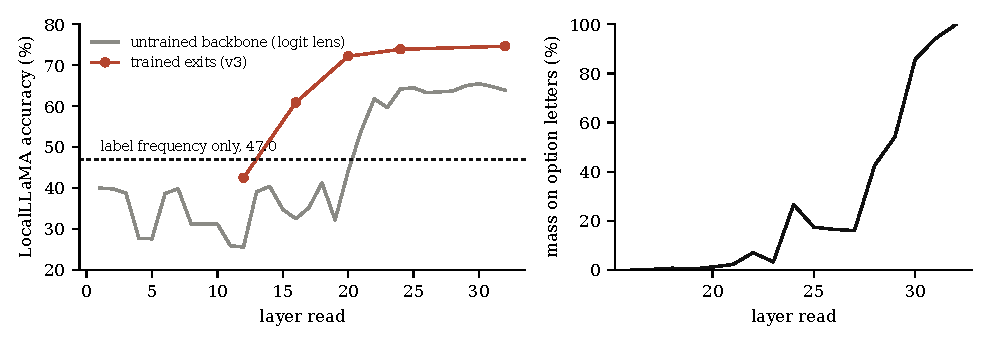
\includegraphics[width=\linewidth]{figures/fig_layers.pdf}
\caption{Left: LocalLLaMA accuracy when the option letters are read at each layer, for the untrained backbone through its own final norm and LM head, and for the trained exits of v3. Right: probability mass on the option letters at each layer of the untrained backbone (JevBench public set).}
\label{fig:layers}
\end{figure}

Each trained exit is an affine map of the residual stream, $\mathrm{norm}(h + Wh + b)$, in the form of a tuned lens~\cite{tunedlens}, with its own logit scale and about 6.5M parameters (26M for the four exits at layers 12, 16, 20 and 24).
Exits read the same LM-head letter rows as the final layer.
They are distilled~\cite{hinton} towards the final layer's answer distribution with detached inputs and separately clipped gradients, so they learn to predict the final answer early without affecting the backbone; full-depth accuracy is the same as without exits.
Each exit has its own temperature, so that a given confidence has the same meaning at every exit; the fitted temperatures lie between 0.78 and 1.04.

At inference the backbone runs in segments (layers 1--12, 13--16, and so on) and keeps the hidden states of all tokens at each segment boundary.
A request stops when the top probability of every question in it reaches a threshold, chosen on the validation split as the lowest value that costs at most about 0.5 points of accuracy (0.86 for v3); this follows the logic of confidence-based early exit~\cite{calm,layerskip}.
A request that does not stop continues from the next layer, so the earlier layers are computed once, and each question costs one additional $2560\times 2560$ multiplication at the exit.
On the validation split, adaptive mode stops at layers 12, 16, 20, 24 and 32 for 4\%, 27\%, 33\%, 11\% and 26\% of questions respectively (22.1 layers on average).
The stopping rule depends on the exit accuracy curve and has to be measured for each version: for an earlier version with exits at layers 12, 16 and 24, choosing between layers 12 and 16 only gave the same accuracy as always using layer 24 at about 60\% of the compute.

\subsection{Training objective and labels}
\label{sec:objective}

The loss is the cross-entropy against a soft target plus 0.5 times the Brier score; score questions add the ranked probability score, so that an error of one level costs less than an error of several.
Soft targets come from five kinds of source: probabilities shipped with public decision datasets; human vote shares with smoothing $(n_k+0.5)/(n+0.5K)$; exactly computed distributions (probability questions, analytic posteriors); structured smoothing for score questions with hard labels, $p(\ell)\propto\exp(-\beta|\ell-\text{gold}|)$ with $\beta$ chosen to give the gold level about 0.7; and label smoothing of 0.05 for the remaining hard labels.
None requires a model call.
The share of soft labels fell from 81\% in the first cloud-trained version, where most came from teacher language models, to about 40\% in v2, and LocalLLaMA KL fell from 0.192 to 0.144 rather than rising.

Options are permuted at random during training, 10\% of questions lose their option descriptions (disabled in v3), and the maximum length is 6,144 tokens.
LoRA~\cite{lora} of rank 16 is applied to all linear layers (attention, Gated DeltaNet projections and MLP).

\subsection{Calibration and a decisive map for yes/no questions}
\label{sec:calib}

An exit's probabilities describe the distribution of annotators or teachers when trained on soft labels, whereas probabilities calibrated on hard labels describe how likely the top option is to be correct.
For an early version with exits at layers 12, 16 and 24, a temperature fitted to argmax hard labels ($T=0.698$) reduced the validation ECE from 0.071 to 0.029 but increased the LocalLLaMA KL from 0.191 to 0.262, while a temperature fitted to soft labels ($T\approx 1.03$) changed neither.
ECE counts the argmax of the soft label as correct, so the closer a model is to the teacher distribution, the more conservative it looks under ECE.
The released model returns the first kind of probability, and all exit temperatures are fitted to soft targets.

JevBench v1.5 scores $P(\text{yes})\in[0.2,0.8]$ as an abstention.
A model trained on soft labels produces intermediate probabilities on contested yes/no questions and loses points under this rule: by argmax 79.7\% of yes/no questions were correct, but 20\% fell in the band.
We fit a monotone map on the unambiguous yes/no questions of the validation split (temperature 0.777, margin 0.2 for v3) that moves probabilities with a clear lean out of the band and leaves genuinely uncertain answers in the middle.
For v3 at full depth it raises Intelligence from 66.9 to 70.1.
Because the map changes the meaning of the returned value, it is an option (enabled by default in the server, disabled with \texttt{--noul calibrated}), and training targets are unchanged.
A zero-shot choice temperature fitted on LocalLLaMA ($T=2.8$) made ECE worse on JevBench, so temperatures must be fitted on held-out data close to the target distribution.

\section{Training}
\label{sec:training}

\subsection{Data}

The training data contains no outputs of the Jev models, no JevBench tasks and no evaluation sets.
From v2 on, it is deduplicated by 13-grams against the LocalLLaMA test set, the JevBench public set and our validation data; the benchmarks in Decision Index are excluded at the source level, and data from the same business workflows as LocalLLaMA is excluded.
Validation splits are grouped by document.
No language model was called to write questions or produce labels for the v2 data.
Table~\ref{tab:data} lists the sources by version.

\begin{table}[t]
\centering\small
\caption{Training data. Question counts are approximate. Each synthetic source is capped at 30k questions.}
\label{tab:data}
\begin{tabular}{p{0.12\linewidth}p{0.80\linewidth}}
\toprule
Version & Sources \\
\midrule
v2 (261k) & Earlier data downsampled to about 60k; public decision-format datasets with program-solved answers; long-document rules (CUAD~\cite{cuad}, MAUD~\cite{maud}, ShARC~\cite{sharc}, LegalBench~\cite{legalbench}); answer judging (PRM800K~\cite{prm800k}, HelpSteer~\cite{helpsteer}, MT-Bench judgements~\cite{mtbench}, SummEval~\cite{summeval}, HaluEval~\cite{halueval}); multi-hop and numeric reasoning (MuSiQue~\cite{musique}, 2WikiMultihopQA~\cite{wiki2}, HotpotQA~\cite{hotpot}, DROP~\cite{drop}, TAT-QA~\cite{tatqa}); natural yes/no (BoolQ~\cite{boolq}, StrategyQA~\cite{strategyqa}, ROPES~\cite{ropes}); human votes (Measuring Hate Speech~\cite{mhs}, SBIC~\cite{sbic}, ChaosNLI over SNLI, MNLI and $\alpha$NLI~\cite{chaosnli,snli,mnli,anli}). \\
v2.1 (+vision) & About 37k image questions: rendered state screenshots (17k), Mind2Web~\cite{mind2web} with Set-of-Mark boxes~\cite{som} (10k), A-OKVQA~\cite{aokvqa} (6k), ScienceQA~\cite{scienceqa} (4k); temporal reasoning in other styles (Test of Time~\cite{tot}, TempReason~\cite{tempreason}). \\
v3 (120k) & Algorithmic conversion of datasets whose answers a program can recompute: FinQA~\cite{finqa} (5.3k), HiTab~\cite{hitab} (1.0k), WikiSQL~\cite{wikisql} (11.8k), ProofWriter~\cite{proofwriter} (20.3k), BoardgameQA~\cite{boardgameqa} (13.0k), and a public decision dataset of published gold and teacher distributions (29.2k); proofs, formulas and programs are never in the input; 62k replay questions and 24k image questions. \\
\bottomrule
\end{tabular}
\end{table}

Distractors for multi-hop and numeric choice questions share the answer's type and are drawn from intermediate-hop answers, entities and numbers in the same passage; for numeric questions from tables they share the answer's unit and magnitude and come from substituting the operation, applying the wrong aggregation or taking neighbouring values.
Several label errors were found during construction, such as HTML-escaped titles that did not match the answer and numeric questions paired with place-name distractors; before the fix 8.1\% of MuSiQue, 5.5\% of HotpotQA and 1.4\% of 2WikiMultihopQA choice questions had two correct options.
Manual inspection of 200 converted items per source found more problems than automated checks did.

\subsection{Versions and recipe}

Table~\ref{tab:versions} summarises the versions and the training recipe.
v0 and v1 used the earlier decision head and are discussed in Section~\ref{sec:neg}.
v2 starts from the post-trained backbone and trains one epoch (16,250 steps of 16 questions, 4.6 hours on one B200) at a learning rate of $10^{-4}$.
Weights are selected by validation loss only; LocalLLaMA and JevBench are used solely to monitor drift.
Every run evaluates at step 0, so problems in the evaluation pipeline surface within minutes.

\begin{table}[t]
\centering\small
\caption{Versions. All use LoRA of rank 16 on all linear layers.}
\label{tab:versions}
\setlength{\tabcolsep}{4pt}\footnotesize
\begin{tabular}{llllll}
\toprule
Version & Readout & Start & Learning rate & Steps $\times$ 16 & Data \\
\midrule
v0 & head, Base & Base & $2\times10^{-4}$ & 3,020 (stopped) & 34k \\
v1 & head, truncated at 24 & Base & $2\times10^{-4}$ & 8,450 & 135k (images) \\
v2 & letters, trained exits & post-trained & $10^{-4}$ & 16,250 & 261k \\
v2.1 & same, vision & v2 & $2\times10^{-5}$ & 7,000 (4,000 chosen) & 164k (120k replay) \\
v3 & same & v2.1 & $10^{-5}$ & 7,500 & 120k (62k replay) \\
\bottomrule
\end{tabular}
\end{table}

v2 met all its predefined criteria: 86.6 on the JevBench public set (at least 85), 72.3 on the hard tier (at least 70), 74.25 on LocalLLaMA (at least 68.0) and KL 0.144 (at most 0.25).
JevBench showed no downward trend during training, and the anchor KL used in earlier experiments was not needed.

\subsection{Forgetting in continued training}

v2.1 adds vision and temporal data to v2.
The first run (learning rate $5\times10^{-5}$, 60k replay questions, 23\% of the total) was stopped at step 2,000: the new data was learnt quickly (Mind2Web from 75\% to 91\%) but v2 validation accuracy fell by 1.7 points and LocalLLaMA by 4.2 points, and was still falling.
The learning rate of v2 had annealed to zero, and raising it again perturbed the existing weights too strongly with too little replay.
The second run lowered the learning rate to $2\times10^{-5}$ and raised replay to 120k questions (74\%), and no further forgetting occurred (Figure~\ref{fig:forgetting}).
Step 4,000 had the lowest validation loss and was selected; between steps 4,000 and 7,000 the paired differences were $-0.2$ [$-0.9$, $+0.4$] on LocalLLaMA and $0.0$ [$-1.3$, $+1.3$] on JevBench.
After vision training, image validation accuracy rose from 75.0 to 91.9 on Mind2Web, from 87.4 to 89.6 on A-OKVQA and from 91.6 to 96.2 on ScienceQA, with text results flat within noise.

\begin{figure}[t]
\centering
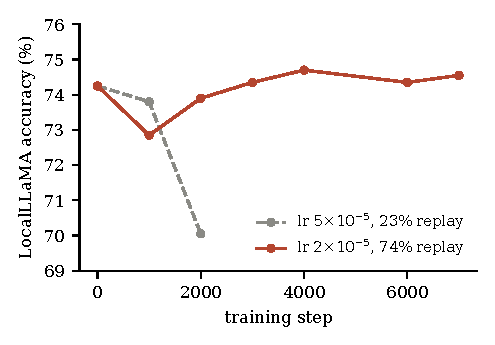
\includegraphics[width=0.5\linewidth]{figures/fig_forgetting.pdf}
\caption{LocalLLaMA accuracy during the two v2.1 runs. A higher learning rate with little replay forgot; a lower rate with mostly replay did not.}
\label{fig:forgetting}
\end{figure}

\subsection{A controlled comparison for hard algorithmic data}
\label{sec:v3}

Performance on the JevBench hard tier remained insufficient through v2.1.
Before the v3 main run, two arms started from v2.1 with a fresh optimizer and trained for 2,000 steps at $10^{-5}$.
The control arm used 24k old text and 6k image questions; the treatment arm used 15.6k old text, about 8.4k new questions and the same 6k image questions.
Weights were selected on the shared validation loss only, with step 0 among the candidates.
The control arm found no weights better than its starting point, so continued training on old data alone brought no gain.
Table~\ref{tab:controlled} shows the paired differences, with confidence intervals from a bootstrap clustered by document or task family.

\begin{table}[t]
\centering\small
\caption{Treatment arm against control arm: accuracy (\%) and paired difference with 95\% interval.}
\label{tab:controlled}
\begin{tabular}{lrrrr}
\toprule
Evaluation & Questions & Control & Treatment & Difference \\
\midrule
held-out algorithmic data, strong distractors & 1,509 & 68.3 & 85.7 & $+17.4$ [14.6, 20.3] \\
held-out algorithmic data, original & 1,508 & 69.9 & 88.8 & $+18.9$ [16.2, 21.6] \\
held-out public decision dataset families & 1,400 & 91.5 & 94.6 & $+3.1$ [1.5, 5.0] \\
original text validation & 5,578 & 87.8 & 87.9 & $+0.1$ [$-0.3$, 0.5] \\
LocalLLaMA & 2,000 & 74.8 & 74.3 & $-0.5$ [$-1.3$, 0.4] \\
\bottomrule
\end{tabular}
\end{table}

The new data produced large gains on its own distribution and no measurable decline on existing abilities.
The v3 main run starts from v2.1 and trains 7,500 steps on this recipe; step 7,500 was selected with validation NLL 0.4011, accuracy 89.43\%, ECE 0.031 and KL 0.226 (Figure~\ref{fig:v3curves}).
Against v2.1 on the same items, v3 improves by 3.7 points [3.1, 4.3] on the full validation split and by 14.1 points [12.0, 16.4] on the held-out new-source data (3,083 questions), and changes by $-0.3$ [$-0.7$, $+0.2$] on the original text validation.
These gains are on the new sources' own distributions; Section~\ref{sec:eval} tests transfer.

\begin{figure}[t]
\centering
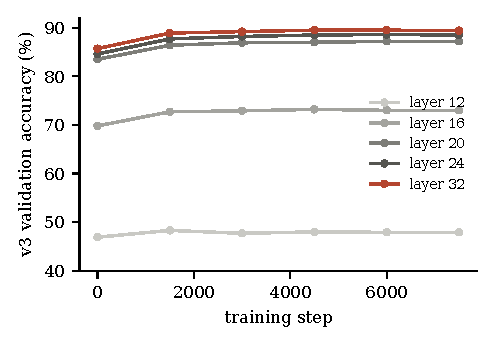
\includegraphics[width=0.5\linewidth]{figures/fig_v3curves.pdf}
\caption{Validation accuracy at each exit during the v3 run (10,209 questions). The validation split includes the new sources, so step 0 (v2.1) scores lower here than on v2.1's own split.}
\label{fig:v3curves}
\end{figure}

\section{Experiments}
\label{sec:eval}

Unless stated otherwise, all results are for the released v3 weights, and no evaluation set was used for training or for weight selection.

\subsection{Main results}

Table~\ref{tab:main} gives the main results.
At full depth v3 reaches 87.4\% on the JevBench public set; the adaptive mode uses 21.6 layers on average at 86.6\%.
On LocalLLaMA the adaptive mode uses about 28 layers with unchanged accuracy (74.65\%) and KL 0.196 against 0.156 at full depth.
For comparison, the dataset card lists 76.8\% for a hosted decision API, 74.2\% for Liquid AI's d1, 72.7\% for Jev 1.13.0 and 67.1\% for an open-weights small model~\cite{localllama,d1,jev}; those figures use a protocol that sends the five questions of a case in one request, whereas ours processes each question as a separate sequence, and our output does not depend on that grouping.

\begin{table}[t]
\centering\small
\caption{Main results of v3 and its predecessors. Intelligence is the JevBench v1.5 score under our scoring, with the decisive yes/no map (default) and without it, in that order.}
\label{tab:main}
\begin{tabular}{lcccc}
\toprule
 & JevBench (231) & JevBench hard (94) & Intelligence & LocalLLaMA \\
\midrule
v3, full depth & \textbf{87.4} & \textbf{75.5} & \textbf{70.1} / 66.9 & \textbf{74.65} (KL 0.156) \\
v3, adaptive & 86.6 & & 68.3 / 65.1 & 74.65 (KL 0.196) \\
v2.1, full depth & 87.0 & 73.4 & 69.0 / 65.8 & 74.7 \\
v2.1, adaptive & 86.1 & & 67.9 / 64.7 & \\
untrained backbone, same prompt & 79.7 & & & 64.1 \\
v1 (decision head) & 74.0 & & & 68.7 \\
\bottomrule
\end{tabular}
\end{table}

\subsection{Open 4B decision models under one protocol}

Each system ran on its authors' server at a fixed revision, each on its own RTX PRO 6000; one client sent identical requests serially and one scorer graded them, with rejected requests counted as errors.
Table~\ref{tab:peers} shows the six systems, where the Trutina column is v2.1 served at full depth (v3 results follow in Section~\ref{sec:paired}).
Trutina has the highest accuracy on LocalLLaMA, this-that and DecisionBench medium, and the lowest median latency; it is the only system of the six that accepts images.
It is weaker on JevBench and much weaker on DecisionBench hard (49.7 against 65.0 for Plumb-4B).
Plumb-4B's published training questions are included in our v2 data, which should be taken into account when comparing.

\begin{table}[t]
\centering\small
\caption{Accuracy (\%) of six open 4B decision models under one protocol. Trutina is v2.1. DB is DecisionBench (state average). JudgeBench counts a pair only if both orders are correct. spark-s1 rejects choice questions with more than about 16 options and answers none of MASSIVE.}
\label{tab:peers}
\begin{tabular}{lcccccc}
\toprule
 & Trutina & JevK5 v0.3 & Plumb-4B & decider-4b & Sieve-4B & spark-s1 \\
\midrule
JevBench public (231) & 87.0 & 89.2 & \textbf{90.0} & 83.1 & 78.4 & 81.0 \\
LocalLLaMA & \textbf{74.7} & 62.5 & 60.8 & 67.7 & 74.1 & 66.9 \\
DB medium & \textbf{82.5} & 80.4 & 82.0 & 74.4 & 72.8 & 38.6 \\
DB hard & 49.7 & 58.4 & \textbf{65.0} & 45.3 & 46.6 & 30.9 \\
this-that & \textbf{51.3} & 47.8 & 48.4 & 47.8 & 45.8 & 43.6 \\
fast-decisions & 61.6 & 62.4 & 61.8 & 61.9 & \textbf{62.9} & 57.4 \\
JudgeBench & 51.3 & 52.1 & 50.3 & \textbf{54.0} & 53.1 & 50.6 \\
MASSIVE & 79.8 & 76.9 & 74.1 & \textbf{88.8} & 84.9 & 0.0 \\
\bottomrule
\end{tabular}
\end{table}

\subsection{Paired comparison of v3 and v2.1}
\label{sec:paired}

Both models were scored on the same items with the same code (6,917 external items, with the tournament for the 132 questions with more than 26 options).
Figure~\ref{fig:paired} shows the paired differences with 95\% intervals from a bootstrap clustered by document or task family.
The gains on JudgeBench ($+3.1$ [1.1, 5.2]) and on inputs over 1,024 tokens ($+0.9$ [0.1, 1.9]) are statistically supported; the gain on DecisionBench hard is not yet confirmed.
Calibration worsened on some external sets: this-that NLL rose from 1.347 to 1.463 and ECE from 0.223 to 0.267, JudgeBench NLL from 0.713 to 0.756 and ECE from 0.160 to 0.180, and LocalLLaMA KL from 0.149 to 0.156.
Our own evaluation had recommended keeping v2.1 as the main version; v3 was nevertheless released as the default, and v2.1 remains available under a version tag.

\begin{figure}[t]
\centering
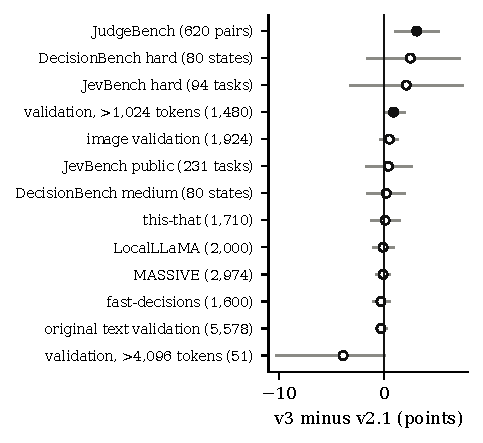
\includegraphics[width=0.62\linewidth]{figures/fig_paired.pdf}
\caption{Paired differences between v3 and v2.1 (points, 95\% intervals). Solid dots: the interval excludes zero. A JudgeBench pair counts only if both orders are correct; only 51 questions exceed 4,096 tokens, hence the wide last interval.}
\label{fig:paired}
\end{figure}

Outside the training distribution, gains over the untrained backbone range from 7 to 9 points: DecisionBench medium 75.2 to 83.3, this-that 43.8 to 51.3 and JudgeBench 46.0 to 54.5.
Accuracy on fast-decisions is unchanged (61.5 to 61.1) while its ECE falls from 0.25 to 0.14.
DecisionBench hard remains below the untrained backbone (53.6 against 52.5).

\subsection{Approximate comparison with 27B models}

Perplexity published per-task accuracy for Jev 1.13.0~\cite{jev}, Qwen3.8-27B~\cite{qwen38} and its own 27B decision model~\cite{pplx} on 11 tasks.
Before running these tasks ourselves, we scanned the public items of each task for 8-gram overlap with all of our training data (an item is a near-duplicate when at least $\max(3,30\%)$ of its 8-grams appear in a single training file).
One task (Circa~\cite{circa}) had 45.8 to 71.5\% near-duplicates depending on the version and was excluded; the 255 near-duplicate items in the remaining tasks were removed, leaving 500 to 1,500 items per task.
The sampled items, prompts and label mappings of the published figures are unavailable, so the comparison is approximate.
Weighted by items, Trutina 4B scores 78.4, Qwen3.8-27B 73.8, the Perplexity 27B model 85.5 and Jev 1.13.0 84.5 (Table~\ref{tab:27b}).
Trutina is ahead of Jev 1.13.0 and Qwen3.8-27B on FinancialPhraseBank and RAGTruth, ahead of all three on ContractNLI, close on Belebele and JevBench hard, and far behind on BBH, WinoGrande and TruthfulQA, which test general knowledge and reasoning.

\begin{table}[t]
\centering\small
\caption{Accuracy (\%) against published figures for 27B models. Trutina: released v3 weights, full depth, default yes/no map. JudgeBench is scored per request (each order separately).}
\label{tab:27b}
\begin{tabular}{lcccc}
\toprule
Task & Trutina 4B & Jev 1.13.0 & Qwen3.8-27B & Perplexity 27B \\
\midrule
FinancialPhraseBank~\cite{fpb} & 82.6 & 77.0 & 75.7 & \textbf{84.2} \\
RAGTruth~\cite{ragtruth} & 79.3 & 77.3 & 61.5 & \textbf{88.8} \\
JevBench public hard & 73.0 & \textbf{73.3} & 72.3 & 70.3 \\
TabFact & 84.8 & 89.8 & 78.6 & \textbf{90.6} \\
ContractNLI & \textbf{84.7} & 77.5 & 80.8 & 80.8 \\
Belebele & 94.6 & \textbf{95.0} & 93.2 & 94.0 \\
WinoGrande~\cite{winogrande} & 72.6 & \textbf{90.7} & 73.1 & 83.3 \\
JudgeBench & 67.1 & \textbf{78.6} & 68.9 & 78.3 \\
BBH & 66.1 & \textbf{94.3} & 72.8 & 82.8 \\
TruthfulQA (binary)~\cite{truthfulqa} & 77.8 & \textbf{92.0} & 82.8 & 85.4 \\
\bottomrule
\end{tabular}
\end{table}

\subsection{Decision Index and image tasks}

The Decision Index 0.3 text public suite score is estimated at about 44 ($\pm 3$) from stratified samples of about 12k rows scored with the official scorer (a full run would take 6 to 8 hours on L4 GPUs).
On the same 2,400 rows v3 scores 44.4 and v2.1 44.7.
The model is strong on tool calling and intent classification (BFCL~\cite{bfcl} 90.6, CLINC150~\cite{clinc} 84.0, BANKING77~\cite{banking} 73.8, API-Bank~\cite{apibank} 81.5, HellaSwag~\cite{hellaswag} 93.8) and scores close to zero on tasks that need multi-step reasoning or specialist knowledge.
On our in-distribution image validation split, accuracy is 93.0 on Mind2Web, 90.2 on A-OKVQA, 98.5 on ScienceQA and 84.9 on rendered workflow screenshots.

\subsection{Zero-shot and training ablations of the readout}
\label{sec:ablate}

We trained four small-scale configurations for 2,000 steps on 1/8 of the v2 data (32k questions) at a learning rate of $10^{-4}$ with the same data and seed.
They were \emph{letters} (train the LoRA and read the option letters, adopted for v2); a \emph{prior plus residual} (PRR), where the LM-head letter logits serve as a prior and the earlier joint head as a zero-initialised residual; an \emph{anchor KL} keeping the output distribution at a few non-answer positions close to the base model~\cite{llmjev}; and a \emph{permutation-consistency} regulariser with a symmetric KL between two option orders of the same question.
All configurations were identical at step 0 (67.7\% on validation), confirming that the residual started from zero (Table~\ref{tab:ablations}).

\begin{table}[t]
\centering\small
\caption{Accuracy (\%) after 2,000 training steps on 32k questions. Untrained: 67.7, 63.9 and 80.5.}
\label{tab:ablations}
\begin{tabular}{lccc}
\toprule
Configuration & v2 validation & LocalLLaMA & JevBench public \\
\midrule
letters & \textbf{83.1} & 73.7 & 81.4 \\
letters + anchor & 81.6 & 71.8 & 81.4 \\
PRR & 83.1 & \textbf{73.8} & 80.1 \\
PRR + anchor & 81.1 & 72.5 & \textbf{83.5} \\
PRR + anchor + consistency & 82.0 & 71.8 & 81.4 \\
\bottomrule
\end{tabular}
\end{table}

A paired bootstrap gives, for letters + anchor against letters, $-1.9$ [$-3.5$, $-0.4$] on LocalLLaMA and $-1.5$ [$-2.3$, $-0.7$] on validation, both significantly worse, and $+0.0$ [$-3.5$, $+3.5$] on JevBench.
PRR against letters is indistinguishable on all three sets.
By question type, PRR was slightly better on score questions ($+1.6$ and $+2.0$) and slightly worse on yes/no ($-0.7$ and $-3.4$), without a net gain, so v2 uses the simplest configuration.
Two points on 231 tasks correspond to about five tasks, so JevBench differences are small relative to their noise.
In these runs JevBench accuracy held or rose with training and the soft-label KL fell from 0.73 to 0.14.

\subsection{Latency}

On one RTX PRO 6000 with serial HTTP requests over the JevBench public set, v3 has a median latency of 19.0~ms at full depth and 14.0~ms in adaptive mode with CUDA graphs~\cite{cudagraphs}, against 29.4 and 20.8~ms eager; means are 38.7 and 30.6~ms, and the p95 (about 110~ms) is set by long-document tasks.
For a single short question latency barely depends on input length; the bottleneck is the overhead of launching kernels layer by layer, which graphs remove, and one graph is captured per exit segment and length bucket.
The median is 12.7~ms when stopping at layer 12 and 29.8~ms through all 32 layers (about 0.86~ms per layer).
Questions with more than 26 options run the tournament and take about 1.2~s at the median and 3.0~s at p95, currently the most significant latency limitation.
On an Apple M5 Pro with MLX~\cite{mlx}, the median is 113~ms at full depth and 71~ms adaptive.
The same model runs on a 16~GB RK3588 board, where a custom bridge sends only the decoder's linear layers to the NPU; because matrix-multiplication time there is far from proportional to matrix size, splitting each layer into tiles with $K\le 3072$ and $N\le 4608$ reduced an adaptive request from 6.0 to 1.7~s (1.2~s with further CPU optimisations), with bit-identical output.
Rockchip's RKLLM~\cite{rknn} runs only full depth and no images.

\section{Negative results and the audit of the first design}
\label{sec:neg}

\paragraph{Decision head on hidden states.}
The first design (v0, v1) followed the pointer head of an earlier decision system: the LM head is removed and a joint decision head (2 layers, 512 dimensions, options attending to one another, 38.2M trainable parameters) is trained on hidden states of a frozen Base backbone with LoRA, with exits at several layers.
It was motivated by linear probes on the layers of frozen Qwen3.5-4B-Base: an ARC~\cite{arc} probe reached 81.7\% at layer 16 and an MMLU~\cite{mmlu} probe 53.9\%, against 52.9 and 46.4 for scoring each option separately, so the middle layers seemed sufficient.
v0 reached 64.2\% on LocalLLaMA after 3,020 steps; v1, trained at larger scale, reached 68.7\% on LocalLLaMA but only 74.0\% on the JevBench public set and 50.5\% on its hard tier, concentrated in long-policy (26\% against 53\% for an open 4B system), multi-hop (56\%) and judging (53\%) families.
The post-trained Qwen3.5-4B read through its own LM head reached 79.7\% without training.
The probe baseline had scored each option separately as \texttt{Answer: <option>}, so the model never saw the options together, and the baseline was correspondingly low.
When all options are shown, the LM head is a strong prior; the new head discarded it and had to relearn answering from over a hundred thousand questions, and the loss was largest outside the training distribution.
Secondary causes were the Base backbone, the removal of the last 8 layers, and the lack of long-document and judging questions.

\paragraph{Training Gated DeltaNet in MLX.}
The Gated DeltaNet layers cannot be trained in MLX as shipped, because the inference kernel has no backward pass and the per-token fallback stores a $[B,32,128,128]$ fp32 state per token (about 16~GB for one layer at $B=8$, $T=1000$).
Following the WY/UT transform~\cite{deltapar} used in flash-linear-attention~\cite{fla}, we implemented a chunked gated delta rule with chunks of 64 tokens, which reduces memory by about 64 times.
The first version inverted the in-chunk triangular system with the product formula
\begin{equation*}
(I+A)^{-1} = \prod_{m=0}^{M-1}\bigl(I + (-A)^{2^m}\bigr),\qquad M=6,
\end{equation*}
whose terms grow like binomial coefficients when neighbouring keys are highly correlated; real data produced NaN at the first step, while tests on random data had not exposed the problem.
A divide-and-conquer inverse that merges blocks level by level has the numerical stability of forward substitution.

\paragraph{Latent reasoning.}
Deep mode was designed as latent reasoning~\cite{coconut,recdepth,pause}: eight latent slots iterate over layers 16 to 24 for $R$ rounds on top of the frozen v1, with a correction added to the layer-24 logits and initialised at zero.
$R=4$ added about 70~ms on the M5 Pro.
On 1,500 validation questions it failed its predefined criterion of clearly outperforming an ensemble over four option orders (Table~\ref{tab:latent}), and training stopped at step 1,000.
Possible causes are that the slots see only what the same frozen layers compute, that many mined hard questions have contested labels, and that the learning rate pushed the correction off course.
The replacement averages over four cyclic permutations of the options; after training its difference from a single full-depth readout was $+0.1$ [$-0.9$, $+1.1$] on 800 choice questions and $+0.7$ [$-2.2$, $+4.3$] on the 139 choice tasks of JevBench, because the position bias~\cite{pride,pine} had largely disappeared.
Deep mode is therefore equivalent to full depth in the released system.

\begin{table}[t]
\centering\small
\caption{Latent deep mode on 1,500 validation questions; ``uncertain'' means a top probability below 0.7 for v1.}
\label{tab:latent}
\begin{tabular}{lcc}
\toprule
 & accuracy, all / uncertain & KL, all / uncertain \\
\midrule
v1, layer 24 & 0.850 / 0.605 & 0.242 / 0.448 \\
option-permutation ensemble (4 orders) & \textbf{0.853 / 0.616} & \textbf{0.241 / 0.442} \\
deep, round 3, step 500 & 0.849 / 0.603 & 0.247 / 0.456 \\
deep, round 3, step 1,000 & 0.851 / 0.610 & 0.243 / 0.450 \\
\bottomrule
\end{tabular}
\end{table}

\paragraph{Self-retrieval reread.}
For long documents we split the input into passages of about 400 characters, read the attention mass of every head~\cite{qrhead} of the 8 full-attention layers on each passage at the answer position (subtracting the attention for an empty question), quoted the four highest-scoring passages before the second copy of the question and read again.
On a held-out part of the long-document validation questions (162) the selected heads gave 74.7\% against 72.2\% for the original readout, but random passages gave the same 74.7\% and JevBench long-document tasks fell from 62.2\% to 56.8\%.
The improvement came from quoting the source again; the evidence was already in context, and the shortcoming was in reasoning with it.

\paragraph{Other methods.}
Permutation consistency on top of the anchor lowered JevBench by 2.1 points; two-letter labels beyond 26 options were 19.9 points below the tournament; 4-bit and 8-bit quantization in MLX made prefill 15 to 25\% slower; and compiling the MLX graph gave no gain.

\section{Limitations}

\paragraph{Hard judgements.}
We analysed the 126 DecisionBench hard questions that v3 answers incorrectly.
Accuracy is 62.5\% on yes/no, 54.3\% on choice and 50.7\% on score questions, and 30 of the 35 score errors are off by one level.
The errors are unrelated to input length (accuracy 80\%, 53\%, 57\% and 59\% for states under 3k characters, 3 to 6k, 6 to 12k and over 12k), the model shows no bias towards yes (it predicts yes for 0.48 of questions against 0.47 in the gold labels), and 45 of the errors have confidence above 0.8.
Typical errors involve multi-step reasoning within the document, such as computing elapsed time from timestamps, tracing a variable through a code change, applying a pinned rule in the presence of a distracting message, and interpreting an inverted grading scale.
Accuracy rises with depth (37.9\% at layer 12 to 57.0\% at layer 32, scored per question), and the last 8 layers still add 3.4 points.
Plumb-4B leads on this evaluation by 12 points. Its training differs from ours: it starts from another trained decision model, mines hard questions with its own model and trains for three epochs on about 3,200 teacher questions the model answers incorrectly or with low confidence plus replay, with questions set in LLM-written business documents solved twice independently.
Our v3 trains for one pass on short, clean algorithmic conversions.
A next step is to mine questions that v3 answers wrongly or with a gold probability below 0.6, mix them with replay and train for two to three epochs.

\paragraph{Arithmetic and calibration.}
Multi-step date and number arithmetic within one forward pass remains weak: JevBench temporal\_numeric stayed at 6 to 7 of 15 tasks from v2 to v3, while the same family in our own data reaches 88\%, so additional data did not resolve it and the problem may require a change in mechanism.
Probabilities are calibrated on our validation mix, and v3 is more confident than v2.1 on some external sets, so applications with high-stakes thresholds should recalibrate.
The training data is almost entirely English.

\paragraph{Contamination.}
Data up to v2 was deduplicated by 13-grams against LocalLLaMA, the JevBench public set and our evaluation sets.
The v3 sources were split from the validation data by document but were not scanned for n-gram overlap with external benchmarks, and the 8-gram scan above ran after training and covers only 11 tasks.
LocalLLaMA and the JevBench public set were used to monitor drift, and JevBench was used to choose the prompt format, so neither is a fully blind evaluation.

\section{Conclusion}

A post-trained 4B backbone read through its own LM head, with a prompt that repeats the question, is a strong typed decision model; trainable exits and a confidence threshold remove about a third of the computation at a cost of 0.8 points on JevBench, and a tournament extends the readout to 255 options without new parameters.
Careful continued training with replay adds capabilities without forgetting, but did not close the gap on multi-step hard judgements, which we regard as the main open problem.
Weights and code are released under Apache-2.0 at \url{https://huggingface.co/aldinelabs/trutina-4b} and \url{https://github.com/aldinelabs/trutina}.

\paragraph{Compute.}
The experiments cost about \$160 of metered cloud compute: the v2 main run \$35, the v3 comparison, training and evaluation \$32, four small-scale ablations \$20, v2.1 (two runs) \$20, v1 training and evaluation \$19, latent reasoning \$7, and other evaluations and measurements \$27.
v0 was trained on a laptop at no cloud cost.

\paragraph{Use of AI assistance.}
An AI coding and writing assistant (Claude, Anthropic) was used in the experiments and in preparing this manuscript.
All arXiv references were checked against arXiv records. The author is responsible for the content.

\bibliographystyle{unsrtnat}
\bibliography{refs}

\end{document}
